\section{Automates ou \textit{Machines d'états Finis} (FSM)}

\begin{frame}{Du circuit au diagramme états-transitions}
  \begin{columns}
    \begin{column}{0.45\textwidth}
      \begin{itemize}
        \item \textbf{Rappel} : les valeurs des sorties $Q$ représentent l'état du système à un instant logique donné.
        \item Le nombre d'états possibles est donc \textbf{fini}.
        \item Il est plus intuitif de les représenter \textit{autrement} :
        \begin{itemize}
          \item \fbox{Diagramme états transitions}
        \end{itemize}
      \end{itemize}
    \end{column}
    \begin{column}{0.55\textwidth}
      \centering
      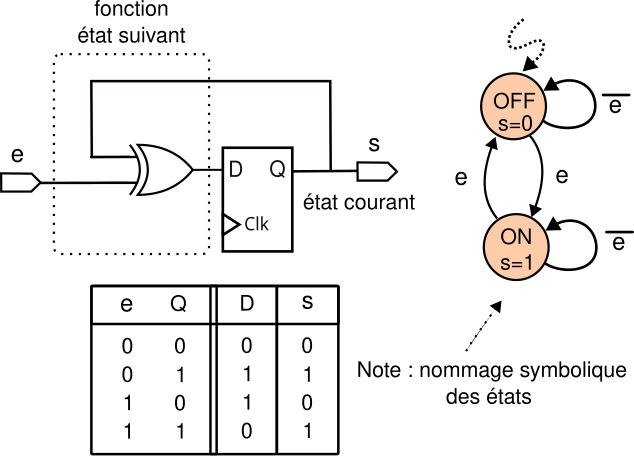
\includegraphics[scale=0.5]{./images/diag_0.png}
    \end{column}
  \end{columns}
\end{frame}


\begin{frame}{Diagramme états-transitions}
  \begin{columns}
    \begin{column}{0.5\textwidth}
      \begin{block}{Définition}
        Un diagramme états-transitions est un \textbf{graphe orienté valué}
        $G = (Q, A)$ où :
        \begin{itemize}
          \item $Q$ : ensemble \textbf{fini} de sommets (les \textit{états}).
          \item $E = \{e_1, \dots, e_n\}$ : signaux d'entrée binaires ;
          $\;\Sigma = \{0,1\}^n$ : espace des combinaisons d'entrée.
          \item $S = \{s_1, \dots, s_m\}$ : signaux de sortie binaires ;
          $\;\Lambda = \{0,1\}^m$ : espace des combinaisons de sortie.
          \item $\mathcal{C} \subseteq \mathcal{P}(\Sigma)$ : ensemble
          de \textit{conditions} (prédicats booléens sur les entrées).
          \item $A \subseteq Q \times \mathcal{C} \times \Lambda \times Q$ :
          ensemble des \textit{arcs orientés}.
        \end{itemize}
      \end{block}
    \end{column}
    \begin{column}{0.5\textwidth}
      \begin{center}
        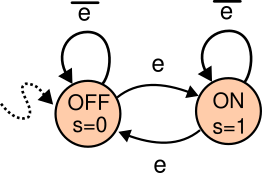
\includegraphics[scale=0.4]{./images/diag_1.png}
      \end{center}
      \begin{center}
      \small
      \textbf{Sémantique d'un arc :} \quad
      $q_i \xrightarrow{\ c\,/\,\lambda\ } q_j
      \;\iff\;
      (q_i,\; c,\; \lambda,\; q_j) \in A$
      \quad avec $c \in \mathcal{C}$
      \end{center}

      \vspace{0.15cm}
      {\small
      \begin{itemize}
        \item $c \in \mathcal{C}$ est un \textbf{prédicat} sur $\Sigma$
          (ex : $e_1 \land \lnot e_2$), permettant \textit{don't-cares}
          et regroupement de combinaisons.
        \item \textbf{Moore} : $\lambda$ dépend uniquement de $q_i$
          (sortie annotée sur le sommet).
        \item \textbf{Mealy} : $\lambda$ dépend de $q_i$ et de la
          combinaison d'entrée effective (sortie annotée sur l'arc).
      \end{itemize}
      }
    \end{column}
  \end{columns}
\end{frame}

%
%
% \begin{frame}{Définition formelle d'un \textbf{automate de Moore}}
%   Une automate de Moore est un sextuplet $(Q, \Sigma, \Delta, \sigma, \lambda, q_0 )$ :
%   \begin{itemize}
%   \item $Q$ est un ensemble fini d’états, $q_0$ est l’état initial
%   \item $\Sigma$ est l’alphabet d’entrée, $\Delta$ est l’alphabet de sortie
%   \item $\delta$ est une application de $Q \times \Sigma $ dans $Q$ : {\it fonction de transition}
%   \item $\lambda$  est une application de $Q$ dans $\Delta$, donnant la sortie associée à chaque état
%   \end{itemize}
%
%   La sortie de l'automate de Moore en réponse à une entrée $a_1 a_2\dots a_n$ , $n \geq 0$ est
%   $\lambda(q_0),\lambda(q_1)\dots \lambda(q_n)$ où
%   $q_0 ,\dots, q_n$ est la séquence d’états tels que $\lambda(q_{i-1},a_i) = q_i$ pour $1 \leq i \leq n$.
%   Remarque: Un automate de Moore retourne la sortie $\lambda(q_0)$ pour toute entrée.
% \end{frame}
%
% \begin{frame}{Définition formelle d'un \textbf{automate de Mealy}}
%   Une automate de Mealy est un sextuplet $(Q, \Sigma, \Delta, \sigma, \lambda, q_0 )$ :
%   \begin{itemize}
%   \item $Q$ est un ensemble fini d’états, $q_0$ est l’état initial
%   \item $\Sigma$ est l’alphabet d’entrée, $\Delta$ est l’alphabet de sortie
%   \item $\delta$ est une application de $Q \times \Sigma $ dans $Q$ : {\it fonction de transition}
%   \item $\lambda$  est une application de $Q\times \Sigma$ dans $\Delta$, donnant la sortie associée à chaque état
%   \end{itemize}
%
%   $\lambda(q, a)$ donne la sortie associée à une transition d’un état q sur l’entrée a.
%   La sortie de l'automate de Mealy,en réponse à une séquence d’entrées $a_1,\dots a_n$ est
%   $\lambda(q_0, a_1) \lambda(q_1 , a_2 ) \dots \lambda(q_{n-1}, a_n)$
%   où $q_0 , q_1 ,\dots, q_n$ est la séquence des états tels que
%   $\lambda(q_{i-1}, a_i) = q_i$ pour $1 \leq i \leq n$.
% \end{frame}

\begin{frame}{Automates de Moore et Mealy : différences électroniques}
  \begin{figure}[h!]
    \centering
    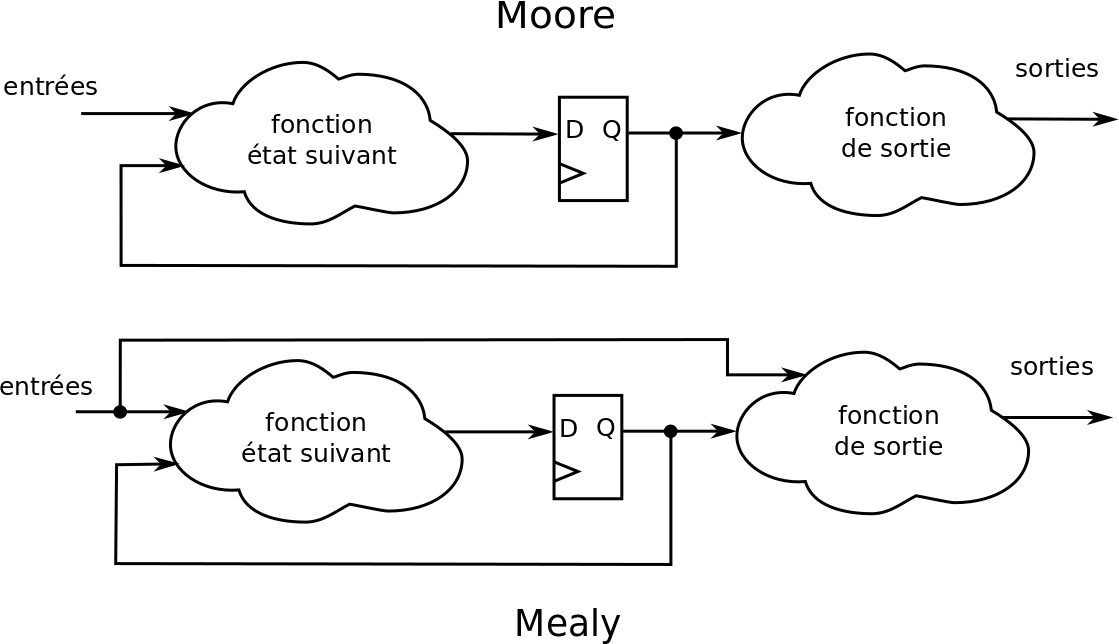
\includegraphics[scale=0.20]{./images/moore_mealy.png}
    %\caption{Automates de Moore et de Mealy}
    %\label{fig:mealy_moore}
  \end{figure}
  \begin{alertblock}{Warnings}
    \begin{itemize}
      \item Composer (i.e interconnecter) des automates de Mealy est \textbf{dangereux}.
      \item Création potentielle de \textbf{boucles combinatoires} : \color{red}{interdit}
    \end{itemize}
  \end{alertblock}
\end{frame}

\begin{frame}{Concevoir un circuit : du diagramme au circuit}
  Un problème de conception d'automate peut se résumer de la manière suivante :
  \begin{enumerate}
    \item Formulation du problème $\rightarrow$ diagramme états-transitions.
    \item Vérification de la {\it causalité} de l'automate décrit.
    \item Encodage des états.
    \item Construction du tableau de séquencement (si nécessaire)
    \item Détermination des fonctions d'état suivant (fonction de transition) et sorties.
  \end{enumerate}

  \begin{figure}[h!]
    \centering
    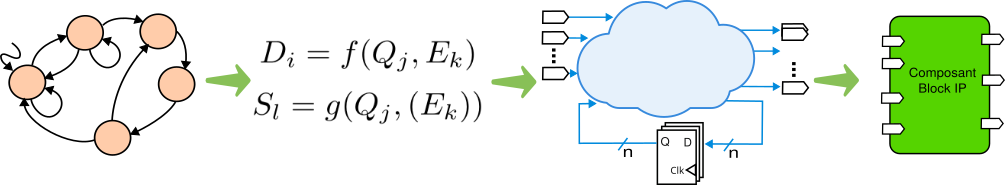
\includegraphics[scale=0.5]{./images/diag_2.png}
    \label{fig:mealy_moore}
  \end{figure}
\end{frame}

\begin{frame}{Vérification de causalité d'un automate}
  \vspace{0.4cm}
  \begin{columns}
    \begin{column}{0.75\textwidth}
      Pour qu'un automate soit considéré comme consistant ou {\it causal}, on doit examiner les conditions $c_i(s)$ des transitions
      partant de chaque état $s\in Q$.
      \begin{itemize}
        \item \textbf{Réactivité} Les conditions sur les transitions doivent être {\it collectivement exhaustives} : il existe forcément une transition à '1'.
        $$\forall s \in Q : \sum_i c_i(s)=1$$
        \item \textbf{Déterminisme} Les conditions sur les transitions doivent être {\it mutuellement exclusives} : on ne peut pas avoir deux transitions à '1' en même temps.
        $$\forall s \in Q, \forall (i,j), i\neq j : c_i(s).c_j(s)=0$$
      \end{itemize}
    \end{column}
    \begin{column}{0.25\textwidth}
      \begin{figure}[h!]
        \centering
        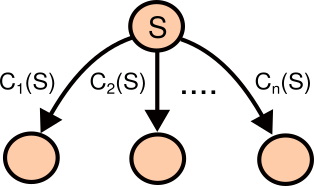
\includegraphics[scale=0.35]{./images/stg_1.png}
      \end{figure}
    \end{column}
  \end{columns}

  \begin{alertblock}{Retenir}
    Cela signifie simplement que dans un état, il existe un, et un seul, état suivant.
  \end{alertblock}

  Notons qu'un état peut avoir comme état suivant lui-même.\\
\end{frame}


\begin{frame}{Etude de cas : vending machine (distributeur)}
  \begin{columns}
    \begin{column}{0.5\textwidth}
      \textbf{Objectif}
      On cherche à réaliser un dispositif qui délivre un objet (cannette etc), après que l'on y a introduit 15 centimes.
      Ces 15 centimes peuvent être introduits à l'aide de pièces de 5 (N) ou 10 centimes (D). La machine ne rend pas la monnaie.
    \end{column}
    \begin{column}{0.5\textwidth}
      \begin{figure}[h]
        \centering
        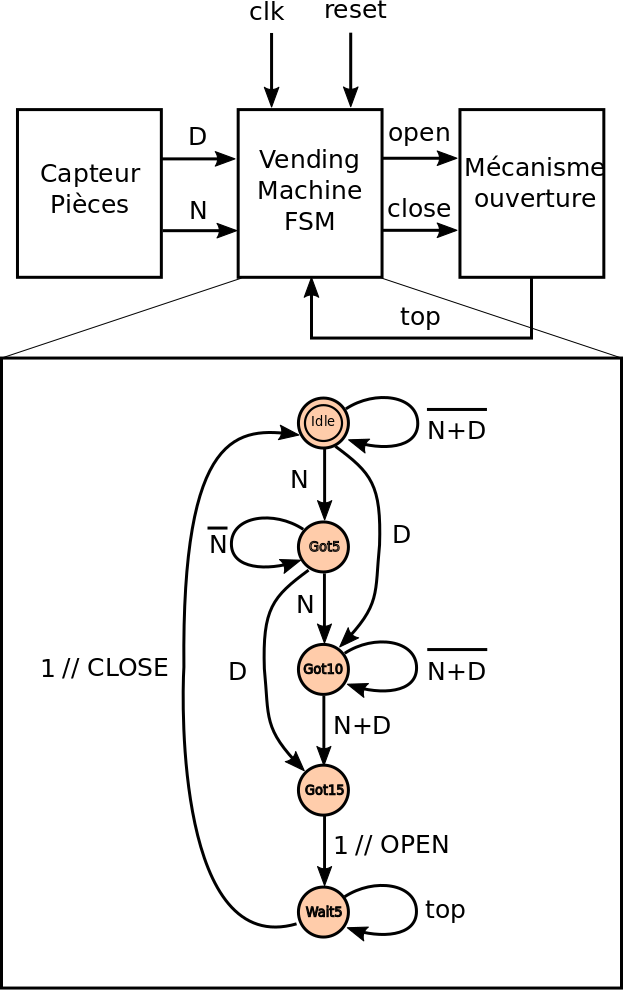
\includegraphics[scale=0.2]{./images/vending_machine.png}
        %\caption{Vending machine et son environnement}
        \label{fig:vending_machine}
      \end{figure}
    \end{column}
  \end{columns}
\end{frame}

\begin{frame}{Etude de cas : encodage des états}
L'encodage des états consiste à associer un code binaire à chaque nom symbolique des états.
  \begin{itemize}
    \item Une infinité d'encodages sont possibles.
    \item Chaque encodage conduit évidemment à des circuits différents structurellement, mais leur comportement
    aux entrées-sorties est identique.
    \item On retiendra \textbf{deux encodages particuliers} :
    \begin{enumerate}
      \item Encodage \textbf{dense} : numérotation binaire classique. Pour $n$ états $\rightarrow$ $\lceil \log_2(n) \rceil$ bits.
      \item Encodage \textbf{"one-hot"} : \textbf{1 bit par état}. $1,2,4,8,16,32,...$. $n$ états $\rightarrow$ $n\rceil$ bits.
    \end{enumerate}
    \item L'encodage "one-hot" permet d'éviter les tableaux de Karnaugh.
  \end{itemize}
\end{frame}

\begin{frame}{Etude de cas : Encodage dense}

  \begin{minipage}{0.4\textwidth}

    \begin{figure}[h]
      \centering
      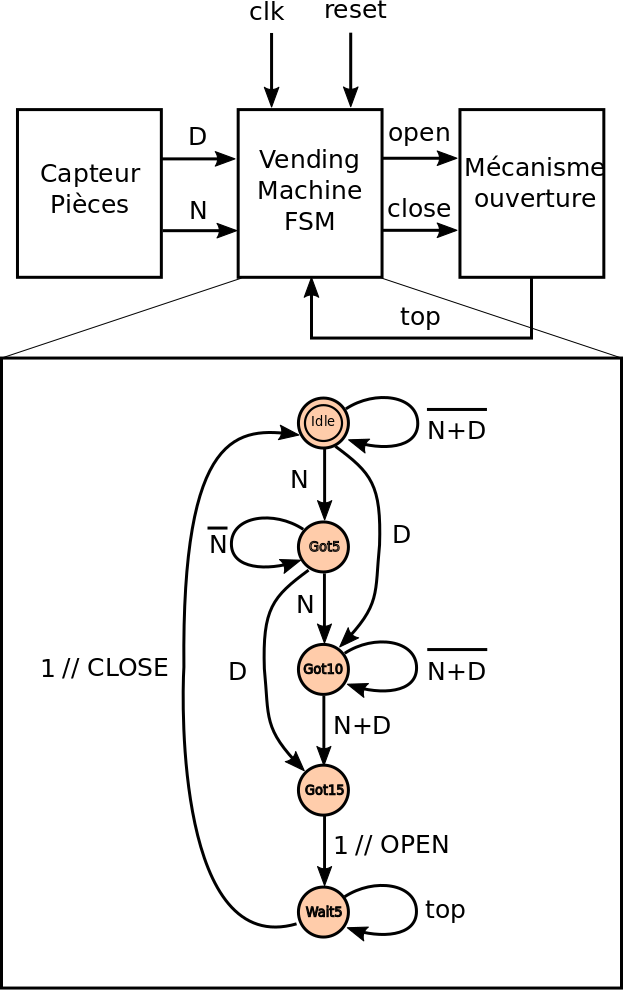
\includegraphics[scale=0.18]{./images/vending_machine.png}
      %\caption{Vending machine et son environnement}
      \label{fig:vending_machine}
    \end{figure}
  \end{minipage}
  \begin{minipage}{0.4\textwidth}
    \begin{table}
      \centering
      Encodage dense :
      \begin{tabular}{|l|c|c|}
            \hline
            état  & numéro & code binaire  \\ \hline \hline
            Idle  & 0      & 000           \\ \hline
            Got5  & 1      & 001           \\ \hline
            Got10 & 2      & 010           \\ \hline
            Got15 & 3      & 011           \\ \hline
            Wait5 & 4      & 100           \\ \hline
        \end{tabular}
    \end{table}
  \end{minipage}


\end{frame}

\begin{frame}{Etude de cas : encodage "one-hot" (1 bit par état)}
  \begin{minipage}{0.4\textwidth}

    \begin{figure}[h]
      \centering
      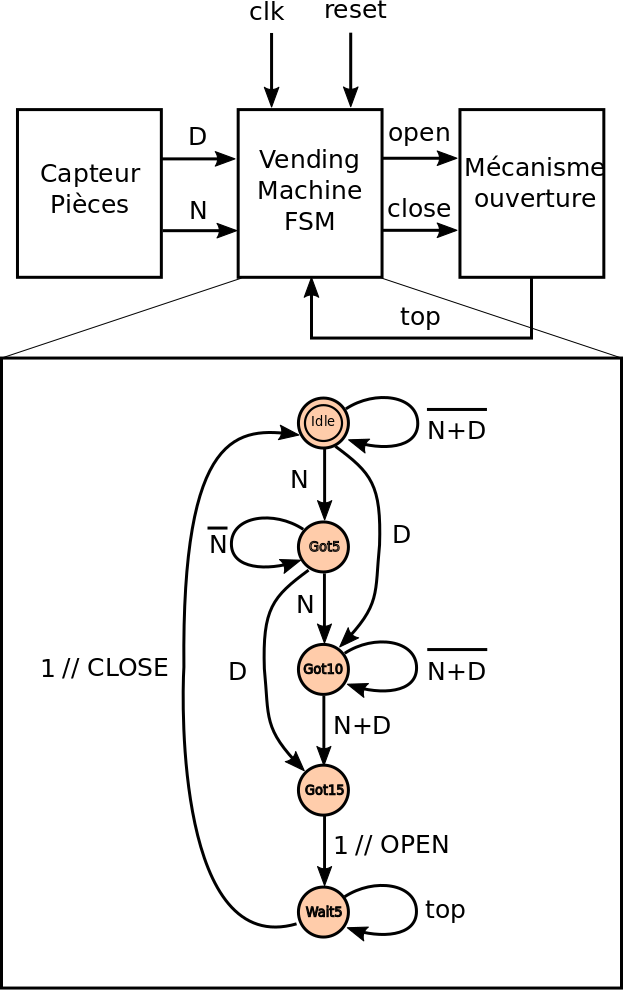
\includegraphics[scale=0.18]{./images/vending_machine.png}
      %\caption{Vending machine et son environnement}
      \label{fig:vending_machine}
    \end{figure}
  \end{minipage}
  \begin{minipage}{0.4\textwidth}
    \begin{table}[!htbp]
      \centering
      Encodage "one-hot" :
      \begin{tabular}{|l|c|c|}
            \hline
            état  & numéro & code binaire  \\ \hline \hline
            Idle  & 1       & 00001           \\ \hline
            Got5  & 2       & 00010           \\ \hline
            Got10 & 4       & 00100           \\ \hline
            Got15 & 8       & 01000           \\ \hline
            Wait5 & 16      & 10000           \\ \hline
        \end{tabular}
    \end{table}
  \end{minipage}
\end{frame}

\begin{frame}{Etude de cas : table de séquencement}
  Le but est de trouver les équations :   $$ D_i=f(Q_j,E_k) $$
    $$ S_l=g(Q_j,(E_k)) $$


Dans un premier temps on conserve les noms des états symboliques.
{\footnotesize
\begin{table}[!htb]
  \centering

  \begin{tabular}{|c|c|c|c||c|c|c|c|}
        \hline
        \cellcolor{blue!25} état courant & $e_1$ & ... & $e_n$ &  \cellcolor{red!25} état suivant & $s_1$ & ... & $s_n$ \\ \hline
        IDLE        & ~    & ~     & ~            & ~            & ~        & ~   & ~    \\ \hline
        \dots       & ~    & ~     & ~            & ~            & ~        & ~   & ~    \\ \hline
        GOT5        & ~    & ~     & ~            & ~            & ~        & ~   & ~    \\ \hline
        \dots       & ~    & ~     & ~            & ~            & ~        & ~   & ~    \\ \hline
    \end{tabular}
\end{table}
}

Puis on utilise l'encodage explicitant les $Q_i$ (état courant) et $D_i$ (état futur).
{\footnotesize
\begin{table}[!htb]
  \centering
    \begin{tabular}{|c|c|c|c|c|c||c|c|c|c|c|c|}
        \hline
        \cellcolor{blue!25}$Q_n$ & \cellcolor{blue!25}\dots & \cellcolor{blue!25} $Q_0$ &  $e_1$ & ... & $e_n$ & \cellcolor{red!25}$D_1$ & \cellcolor{red!25}\dots & \cellcolor{red!25}$D_0$ & $s_1$ & ... & $s_n$ \\ \hline
        ~   & ~    & ~  & ~  & ~  & ~  & ~  & ~  & ~        & ~   & ~ & ~        \\
        ~   & ~    & ~  & ~  & ~  & ~  & ~  & ~  & ~        & ~   & ~ & ~        \\
        \hline
    \end{tabular}
\end{table}
}
\textbf{Equations finales : }
Il reste à observer les colonnes des $D_i$ et $s_j$ et déduire les équations logiques
  \begin{itemize}
    \item Déduction immédiate dans certains cas.
    \item Construction des tableaux de Karnaugh pour chaque $D_i$ et $s_j$
  \end{itemize}
\end{frame}

%
% \begin{frame}{Bascule D : Reset et Set \textit{asynchrones}}
% \begin{columns}
%   \begin{column}{0.45\textwidth}
%     \begin{block}{Cas du \texttt{Reset} : mise à 0}
%       \begin{itemize}
%         \item Le \texttt{reset} est \textbf{prioritaire} sur l'horloge.
%         \item Lorsqu'il est activé $\rightarrow Q=0$
%       \end{itemize}
%     \end{block}
%     \begin{exampleblock}{Cas du \texttt{Set} : mise à 1}
%       \begin{itemize}
%         \item Le \texttt{set} est \textbf{prioritaire} sur l'horloge.
%         \item Lorsqu'il est activé $\rightarrow Q=1$
%       \end{itemize}
%     \end{exampleblock}
%     En cas d'ordres contradictoires $\rightarrow$ voire doc constructeur.
%
%   \end{column}
%   \begin{column}{0.45\textwidth}
%     \centering
%     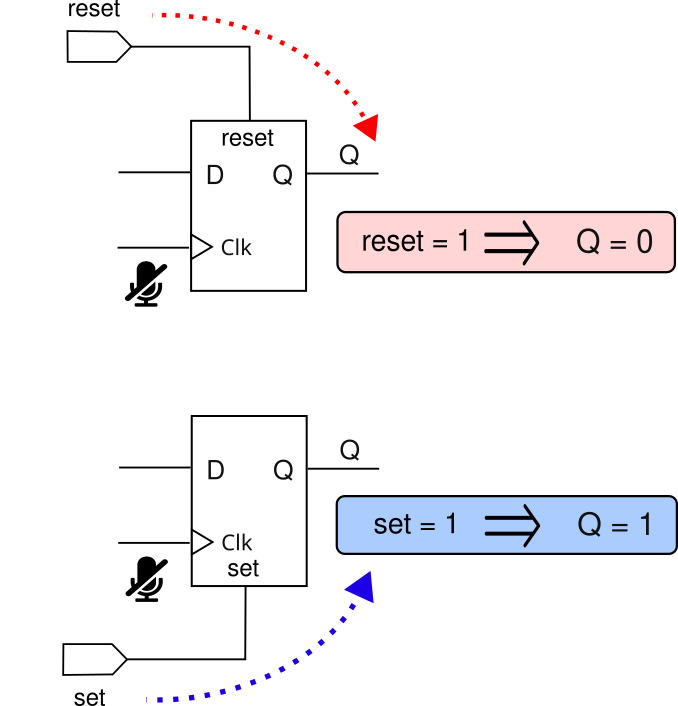
\includegraphics[scale=0.4]{./images/reset_0.png}
%   \end{column}
% \end{columns}
% \end{frame}
%
% \begin{frame}{Bascule D : Reset et Set \textit{asynchrones}}
% \begin{columns}
%   \begin{column}{0.40\textwidth}
%     \centering
%     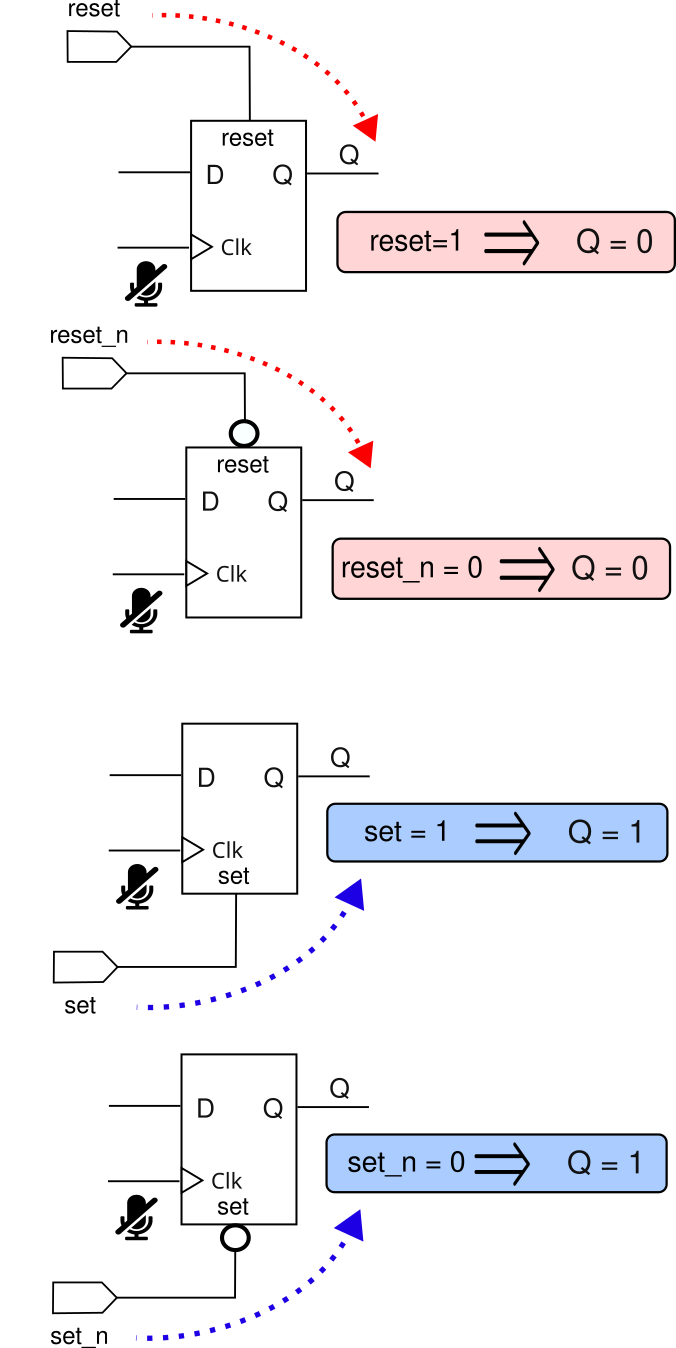
\includegraphics[scale=0.21]{./images/reset_1.png}
%   \end{column}
%   \begin{column}{0.55\textwidth}
%     \begin{block}{Polarité d'activation}
%       \begin{itemize}
%         \item  Les deux signaux \texttt{reset} et \texttt{set} ont eux-mêmes une valeur où ils sont
%         actifs.
%         \item Cette valeur est précisée dans le schéma de la bascule :
%         \begin{itemize}
%           \item Cerle ° indique la \fbox{polarité \texttt{0} active}.
%           \item L'\underline{absence de cercle} ° indique la \fbox{polarité \texttt{1} active}.
%         \end{itemize}
%         \item Cette valeur \textit{peut} être précisée dans le \textit{nommage} du signal :
%         \begin{itemize}
%           \item \texttt{reset\_n} indique une polarité \texttt{0} active.
%           \item \texttt{reset} indique une polarité \texttt{1} active.
%         \end{itemize}
%       \end{itemize}
%     \end{block}
%     \begin{itemize}
%       \item Les noms des signaux dépendent des \textit{conventions de nommage} propres aux entreprises.
%       \item \textbf{Attention : } bien connecter \textbf{tous} les \texttt{reset} et \texttt{set}.
%     \end{itemize}
%   \end{column}
% \end{columns}
% \end{frame}

\begin{frame}{Cas d'étude : automate \texttt{ABC}}
    \begin{columns}
        \begin{column}{0.5\textwidth}

            \begin{center}
              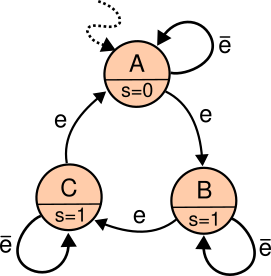
\includegraphics[scale=0.35]{./images/diag_5.png}
            \end{center}
            \centering
            \vspace{0.2cm}

            \begin{tabular}{|c|c||c|c|}
                \hline
                \textbf{État courant} & \(e\) & {\textbf{État futur}} & \(S\) \\
                \hline
                A & 0 & A & 0 \\
                A & 1 & B & 0 \\ \hline
                B & 0 & B & 1 \\
                B & 1 & C & 1 \\ \hline
                C & 0 & C & 1 \\
                C & 1 & A & 1 \\
            \hline
            \end{tabular}
        \end{column}

        \begin{column}{0.5\textwidth}
            \centering
            \textbf{Encodage} : A $\leftrightarrow$ \texttt{00},B $\leftrightarrow$ \texttt{01},C $\leftrightarrow$ \texttt{10}
            %\renewcommand{\arraystretch}{1.3}
            \begin{tabular}{|c|c|c||c|c|c|}
                \hline
                \multicolumn{2}{|c|}{\textbf{État courant}} & \textbf{Entrée}
                & \multicolumn{2}{c|}{\textbf{État futur}} & \textbf{Sortie} \\
                \hline
                \(Q_1\) & \(Q_0\) & \(e\) & \(D_1\) & \(D_0\) & \(S\) \\
                \hline
                0 & 0 & 0 & 0 & 0 & 0 \\
                0 & 0 & 1 & 0 & 1 & 0 \\ \hline
                0 & 1 & 0 & 0 & 1 & 1 \\
                0 & 1 & 1 & 1 & 0 & 1 \\ \hline
                1 & 0 & 0 & 1 & 0 & 1 \\
                1 & 0 & 1 & 0 & 0 & 1 \\
            \hline
            \end{tabular}

            \[
              \left\{
              \begin{aligned}
              D_1 &= \overline{Q_1}.Q_0.e+Q_1.\overline{Q_0}.\overline{e}\\
              D_0 &= \overline{Q_1}.\overline{Q_0}.e + \overline{Q_1}.Q_0.\overline{e}\\
              S   &= Q_1 \oplus Q_0\\
              \end{aligned}
              \right.
            \]

            Il nous manque une technique pour faire mieux : les \textbf{Don't care}
        \end{column}
    \end{columns}
\end{frame}

\begin{frame}{Techniques des \textbf{Don't cares} : profiter des indéterminations}
  \begin{block}{Don't cares}
    \begin{itemize}
      \item Cas manquants, non-applicables $\rightarrow$ sources d'optimisations booléennes.
      \item Présentés comme des \textbf{valeurs libres} '\texttt{X}' (ou '\texttt{-}') dans le tableau de Karnaugh.
    \end{itemize}
  \end{block}

  \begin{columns}
      \begin{column}{0.55\textwidth}
        \begin{tabular}{|c|c|c||c|c|c|}
                \hline
                \multicolumn{2}{|c|}{\textbf{État courant}} & \textbf{Entrée}
                & \multicolumn{2}{c|}{\textbf{État futur}} & \textbf{Sortie} \\
                \hline
                \(Q_1\) & \(Q_0\) & \(e\) & \(D_1\) & \(D_0\) & \(S\) \\
                \hline
                0 & 0 & 0 & 0 & 0 & 0 \\
                0 & 0 & 1 & 0 & 1 & 0 \\ \hline
                0 & 1 & 0 & 0 & 1 & 1 \\
                0 & 1 & 1 & 1 & 0 & 1 \\ \hline
                1 & 0 & 0 & 1 & 0 & 1 \\
                1 & 0 & 1 & 0 & 0 & 1 \\ \hline
                1 & 1 & 0 & x & x & x \\
                1 & 1 & 1 & x & x & x \\
            \hline
            \end{tabular}
      \end{column}
      \begin{column}{0.4\textwidth}
        \textbf{D1 :}
        \begin{tabular}{|c|c|c|}
          \hline
          \diagbox{$Q_1Q_0$}{$e$} & 0 & 1 \\
          \hline
          00 & ~ & ~ \\
          \hline
          01 & ~ & \cellcolor{blue!25}1 \\
          \hline
          11 & \cellcolor{red!30}x & \cellcolor{blue!25}x \\
          \hline
          10 & \cellcolor{red!30}1 & ~ \\
          \hline
        \end{tabular}\\

        \textbf{D0 :}
        \begin{tabular}{|c|c|c|}
          \hline
          \diagbox{$Q_1Q_0$}{$e$} & 0 & 1 \\
          \hline
          00 & ~ & 1 \\
          \hline
          01 & \cellcolor{red!30}1 & ~ \\
          \hline
          11 & \cellcolor{red!30}x & x \\
          \hline
          10 & ~ & ~ \\
          \hline
        \end{tabular}
      \end{column}
  \end{columns}
\end{frame}

\begin{frame}{Cas d'étude : automate \texttt{ABC}}
  \begin{columns}
    \begin{column}{0.4\textwidth}
      \textbf{Diagramme états-transitions}
      \begin{center}
        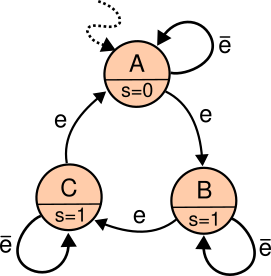
\includegraphics[scale=0.35]{./images/diag_5.png}
      \end{center}

      \textbf{Equations constitutives :}
      \begin{itemize}
        \item Choix : encodage dense
        \item Longs calculs...
      \end{itemize}
      \[
        \left\{
          \begin{aligned}
          D_1 &= Q_0.e+Q_1.\overline{e}\\
          D_0 &= Q_0.\overline{e}+ \overline{Q_1}.\overline{Q_0}.e \\
          S   &= Q_1 \oplus Q_0\\
          \end{aligned}
          \right.
      \]
    \end{column}
    \begin{column}{0.6\textwidth}
      \textbf{Circuit numérique}
      \begin{center}
        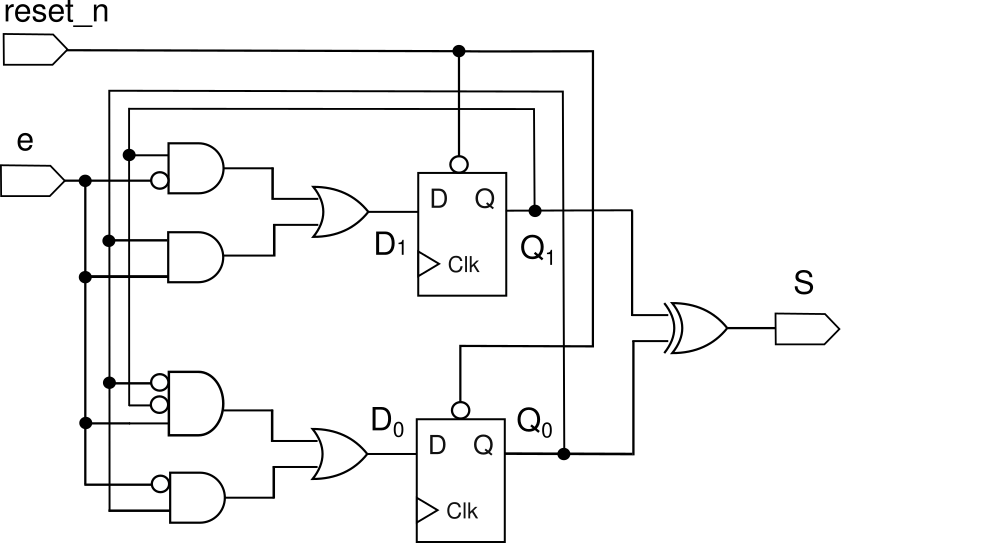
\includegraphics[scale=0.30]{./images/abc.png}
      \end{center}
    \end{column}
  \end{columns}
\end{frame}

\begin{frame}{Cas \textit{Merveilleux} de l'encodage One-Hot}

On peut déduire les équations \textbf{directement} par simple \textbf{lecture} du diagramme états-transitions.

\begin{alertblock}{Principe}
  \begin{itemize}
    \item Cet encodage spécifique signifie qu'\textbf{une seule} bascule $D_i$ présente une sortie $Q_i$ à $1$.
    \item Tout se passe donc comme si un \textbf{jeton} circule d'\textbf{une bascule à l'autre}.
    \item Savoir quelle bascule "détient le jeton" suffit à connaître l'état courant.
  \end{itemize}
\end{alertblock}

\textbf{Application directe} du schéma de traduction suivant :
\begin{columns}
  \begin{column}{0.5\textwidth}
    \begin{figure}[!htp]
      \centering
      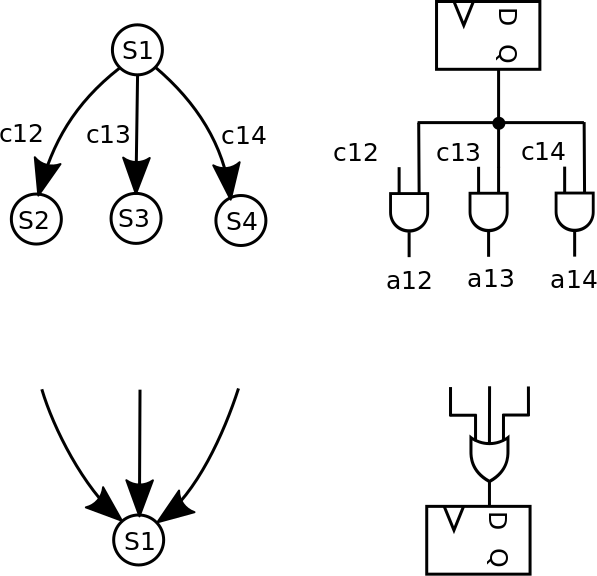
\includegraphics[scale=0.16]{./images/one_hot_method.png}
      %\caption{Procédé simplifiant la génération d'un circuit d'automate dans le cas d'un encodage {\it one-hot}.}
      \label{fig:one_hot}
    \end{figure}
  \end{column}

  \begin{column}{0.5\textwidth}
    \begin{equation*}
      \begin{cases}
        d_2=q_1.c_{12}+\dots \\
        d_3=q_1.c_{13}+\dots \\
        d_4=q_1.c_{14}+\dots \\
        d_1=\dots + \dots + \dots \\
      \end{cases}
    \end{equation*}
  \end{column}
\end{columns}
\end{frame}

%================================================================
\begin{frame}{Encodage one-hot : exemple sur l'automate \texttt{ABC}}
  \begin{columns}
    \begin{column}{0.5\textwidth}
      \centering
      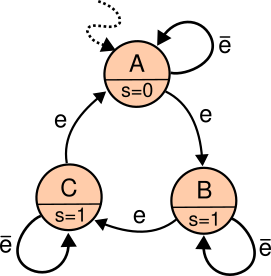
\includegraphics[scale=0.35]{./images/diag_5.png}
      \begin{itemize}
        \item Application du schéma de traduction :
      \end{itemize}
      \begin{columns}
        \begin{column}{0.5\textwidth}
          \begin{figure}[!htp]
            \centering
            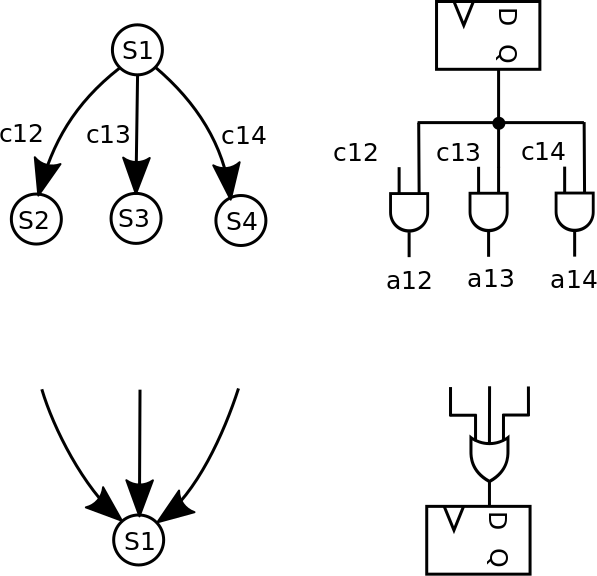
\includegraphics[scale=0.12]{./images/one_hot_method.png}
            %\caption{Procédé simplifiant la génération d'un circuit d'automate dans le cas d'un encodage {\it one-hot}.}
            \label{fig:one_hot}
          \end{figure}
        \end{column}

        \begin{column}{0.5\textwidth}
          \begin{equation*}
            \begin{cases}
              D_0=Q_0.\overline{e}+Q_2.e \\
              D_1=Q_1.\overline{e}+Q_0.e  \\
              D_2=Q_2.\overline{e}+Q_1.e  \\
              S=Q_1 + Q_2\\
            \end{cases}
          \end{equation*}
          {\scriptsize Note : le calcul de \texttt{S} est hors schéma.}
        \end{column}
      \end{columns}
    \end{column}
    \begin{column}{0.5\textwidth}
      \begin{figure}[!htp]
        \centering
        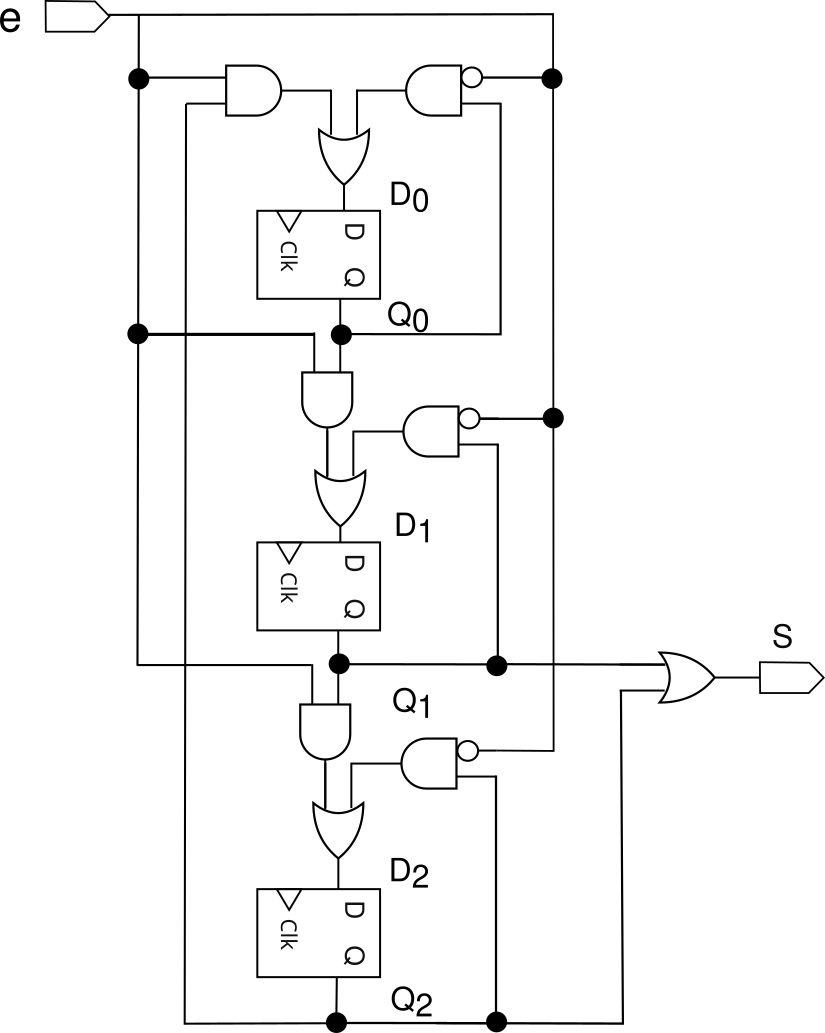
\includegraphics[scale=0.22]{./images/abc_one_hot.png}
        %\caption{Procédé simplifiant la génération d'un circuit d'automate dans le cas d'un encodage {\it one-hot}.}
        %\label{fig:one_hot}
      \end{figure}
    \end{column}
  \end{columns}
\end{frame}

\begin{frame}{Encodage one-hot : exemple sur l'automate \texttt{ABC}}
  \begin{columns}
    \begin{column}{0.5\textwidth}
      \textbf{Initialisation du circuit : en \color{red}{rouge}}
      \begin{itemize}
        \item Etat initial attendu : $A \rightarrow 001$
        \item Le signal \texttt{reset\_n} est \textbf{actif bas}.
        \begin{itemize}
          \item Nommage "\texttt{\_n}" (convention).
        \end{itemize}
        \item $Q_0$ doit valoir 1 : on utilise la "patte" \texttt{set}.
        \begin{itemize}
          \item ici active à 0 (présence '°' indiquée sur la bascule)
        \end{itemize}
        \item $Q_1$ doit valoir 0 : on utilise la "patte" \texttt{reset}.
        \item $Q_2$ doit valoir 0 : on utilise la "patte" \texttt{reset}.
        \begin{itemize}
          \item ici active à 0 (présence '°' indiquée sur la bascule)
        \end{itemize}
      \end{itemize}
      \textbf{Autres câblages : }
      \begin{itemize}
        \item \textbf{Désactivation} ({\color{blue}{bleu}}) des \texttt{reset} et \texttt{set} inutilisés.
        \item \color{black}Présence de l'horloge en \color{green}{vert}.
        % \item Notez l'absence des signaux d'alimentation des portes logiques.
        % \begin{itemize}
        %   \item Mais cette alimentation existe bien !
        % \end{itemize}
      \end{itemize}
    \end{column}
    \begin{column}{0.5\textwidth}
      \begin{figure}[!htp]
        \centering
        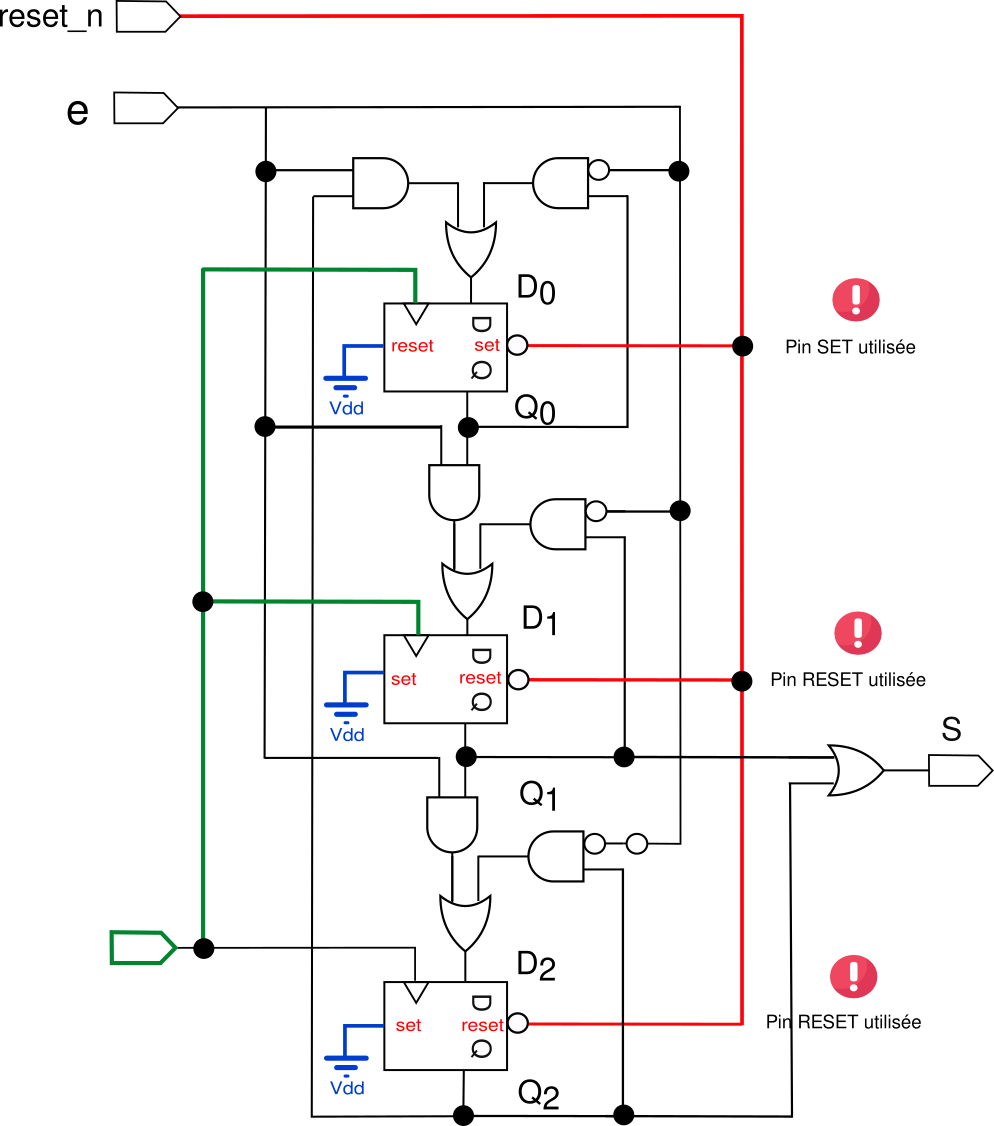
\includegraphics[scale=0.22]{./images/abc_one_hot_reset.png}
        %\caption{Procédé simplifiant la génération d'un circuit d'automate dans le cas d'un encodage {\it one-hot}.}
        %\label{fig:one_hot}
      \end{figure}
    \end{column}
  \end{columns}

\end{frame}

% \begin{frame}{Cas de l'encodage One-Hot}
%
%   \begin{itemize}
%     \item On dessine une bascule $D$ pour un état $S$
%     \item Pour chacune des transitions sortantes d'un état $S_i$ vers un état $S_j$, on dessine une porte AND connectée d'une part à la sortie $Q$ de la bascule de l'état $S_i$, et
%     d'autre part la condition booléenne $c$ de la transition $S_i\rightarrow_{c} S_j$. Appelons $c_{i,j}$ la sortie de cette porte AND.
%     \item Pour chacune des transitions entrantes d'un état $S_j$ on dessine une porte OR connectée à l'entrée $D_j$ et possédant autant d'entrées qu'il existe de transitions entrantes.
%     A partir des états précedents $S_i$, on connecte le signal $c_{i,j}$ sur une des entrées de cette porte OR.
%   \end{itemize}
%
% \end{frame}


\begin{frame}{Rappel}
\begin{itemize}
  \item Dans certains cas simples, il reste possible de dessiner le circuit.
  \item Sinon, on s'en tient au schéma d'ensemble suivant :
\end{itemize}

\begin{figure}[!htp]
  \centering
  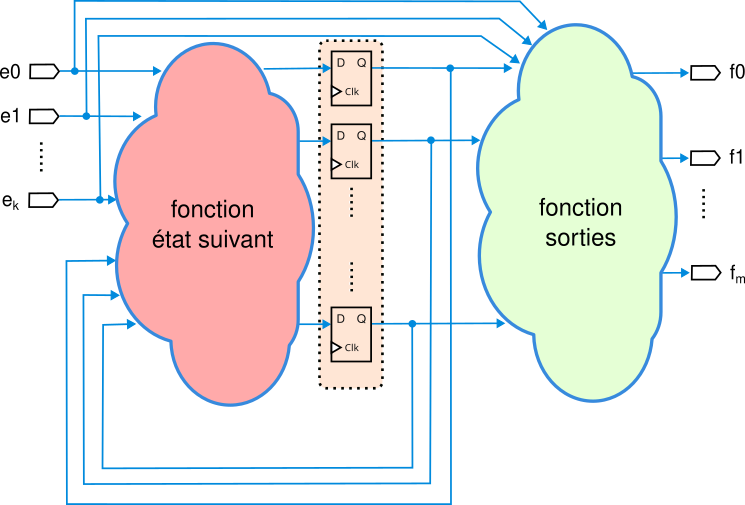
\includegraphics[scale=0.4]{./images/fsm_4.png}
  %\caption{Procédé simplifiant la génération d'un circuit d'automate dans le cas d'un encodage {\it one-hot}.}
  %\label{fig:one_hot}
\end{figure}

\end{frame}
